\documentclass{article}

% if you need to pass options to natbib, use, e.g.:
\PassOptionsToPackage{numbers, compress}{natbib}
% before loading nips_2018

% ready for submission
\usepackage{nips_2018}

\usepackage[utf8]{inputenc} % allow utf-8 input
\usepackage[T1]{fontenc}    % use 8-bit T1 fonts
\usepackage{booktabs}       % professional-quality tables
\usepackage{amsfonts}       % blackboard math symbols
\usepackage{nicefrac}       % compact symbols for 1/2, etc.
\usepackage{microtype}      % microtypography

\usepackage{mathrsfs}
\usepackage{graphicx}
\usepackage{xr-hyper} % cross-references (between documents)
\usepackage{xcolor} % Allow colors to be defined
\usepackage{geometry} % Used to adjust the document margins
\usepackage{amsmath} % Equations
\usepackage{amssymb} % Equations
% The hyperref package gives us a pdf with properly built
% internal navigation ('pdf bookmarks' for the table of contents,
% internal cross-reference links, web links for URLs, etc.)
\usepackage[hyphens]{url}
\usepackage[hypertexnames=false]{hyperref}
\usepackage[title,toc]{appendix}
\usepackage{natbib}
\usepackage{bm}
\usepackage{mathtools}
\usepackage{rotating,tabularx}

% Nicer default font (+ math font) than Computer Modern for most use cases
\usepackage{mathrsfs}
\usepackage{graphicx}
\usepackage{xr-hyper} % cross-references (between documents)
\usepackage{xcolor} % Allow colors to be defined
\usepackage{geometry} % Used to adjust the document margins
\usepackage{amsmath} % Equations
\usepackage{amssymb} % Equations
% Colors for the hyperref package
% The hyperref package gives us a pdf with properly built
% internal navigation ('pdf bookmarks' for the table of contents,
% internal cross-reference links, web links for URLs, etc.)
\usepackage{hyperref}
\usepackage[title,toc]{appendix}
\hypersetup{
    colorlinks=true,
    pdfborder=0 0 1,
    pdftitle=\georddtitle{},
    allcolors=[rgb]{0.00,0.38,0.59},
    allbordercolors=[rgb]{0.60,0.76,0.86}
}
\usepackage{natbib}
\usepackage{bm}
\usepackage{mathtools}
\usepackage{pdflscape}
\usepackage[doublespacing,nodisplayskipstretch]{setspace}
% only use if doublespacing:
\renewcommand*{\arraystretch}{0.8} % https://tex.stackexchange.com/questions/183562/how-to-reduce-vertical-space-in-matrix
\def\SmallColSep{\setlength{\arraycolsep}{3pt}}
% \usepackage{authblk}

\usepackage{enumitem}
\newlist{flatlist}{enumerate*}{1}
\setlist[flatlist]{label=(\arabic*)}


\newcommand{\mathbold}[1]{\bm{#1}} % if not using mathpazo

\DeclarePairedDelimiter{\parenthesis}{\lparen}{\rparen}
\DeclarePairedDelimiter{\squarebracket}{\lbrack}{\rbrack}
\DeclarePairedDelimiter{\curlybracket}{\lbrace}{\rbrace}
\DeclarePairedDelimiter{\absolutevalue}{\lvert}{\rvert}
\newcommand{\del}[1]{\parenthesis*{#1}}
\newcommand{\sbr}[1]{\squarebracket*{#1}}
\newcommand{\cbr}[1]{\curlybracket*{#1}}
\newcommand{\abs}[1]{\absolutevalue*{#1}}
% \DeclareMathOperator{\dif}{d}
\newcommand*{\diffdchar}{d}
\newcommand*{\dif}[1]{\mathop{\diffdchar #1}}
\DeclareMathOperator*{\argmin}{arg\,min}
\DeclareMathOperator*{\argmax}{arg\,max}
\let\Pr\relax
\DeclareMathOperator{\Pr}{\mathbb{P}}
\DeclareMathOperator{\E}{\mathbb{E}}
\DeclareMathOperator{\V}{\mathbb{V}}
\DeclareMathOperator{\cov}{{Cov}}
\DeclareMathOperator{\var}{{var}}
\DeclareMathOperator{\Ind}{\mathbb{I}}
\DeclareMathOperator*{\sgn}{{sgn}}

\DeclareMathOperator{\normal}{\mathcal{N}}
\DeclareMathOperator{\unif}{Uniform}
\DeclareMathOperator{\invchi}{\mathrm{Inv-\chi}^2}
\DeclareMathOperator{\ones}{\mathbf{1}}
\DeclareMathOperator{\GP}{\mathcal{GP}}
\newcommand{\building}{\mathtt{BuildClass}}
\newcommand{\district}{\mathtt{Distr}}

% \newcommand*{\trans}{^{\intercal}}
\newcommand*{\trans}{^{\top}}

\newcommand*{\area}{\mathcal{A}}
\newcommand*{\treat}{\mathrm{T}}
\newcommand*{\ctrol}{\mathrm{C}}
\newcommand*{\treatind}{Z}
\newcommand*{\treatarea}{\area{}^{\treat}}
\newcommand*{\ctrolarea}{\area{}^{\ctrol}}

\newcommand*{\sigmaf}{\sigma_{\mathrm{GP}}}
\newcommand*{\sigman}{\sigma_{\epsilon}}
\newcommand*{\sigmabeta}{\sigma_{\beta}}
\newcommand*{\sigmamu}{\sigma_{\mu}}
\newcommand*{\svec}{\mathbold{s}}
\newcommand*{\dvec}{\mathbold{d}}
\newcommand*{\wvec}{\mathbold{w}}
\newcommand*{\yvec}{\mathbold{y}}
\newcommand*{\Yvec}{\mathbold{Y}}
\newcommand*{\yt}{\Yvec_{\treat}}
\newcommand*{\yc}{\Yvec_{\ctrol}}
\newcommand*{\vvec}{\mathbold{v}}
\newcommand*{\muvec}{\mathbold{\mu}}
\newcommand*{\betavec}{\mathbold{\beta}}
\newcommand*{\residvec}{\mathbold{R}}
\newcommand*{\indep}{\protect\mathpalette{\protect\independenT}{\perp}}
\def\independenT#1#2{\mathrel{\rlap{$#1#2$}\mkern2mu{#1#2}}}
\newcommand*{\iid}{iid}
\newcommand*{\vectreat}{\Ind_{T}}

\newcommand*{\border}{\mathcal{B}}
\newcommand*{\sentinel}{\mathbold{b}}
\newcommand*{\numsent}{R}
\newcommand*{\sentinels}{\sentinel_{1:\numsent}}
\newcommand*{\isent}{r}
\newcommand*{\sentinelset}{\cbr{\sentinel_1,\ldots,\sentinel_\numsent}}

\newcommand*{\eye}{\mathbf{I}}

\DeclareMathOperator{\trace}{trace}
\newcommand*{\tauw}{\tau^{w}}
\newcommand*{\unifavg}{\tau^{\mathrm{UNIF}}}
\newcommand*{\invvar}{\tau^{\mathrm{INV}}}
\newcommand*{\taurho}{\tau^{\rho}}
\newcommand*{\tauproj}{\tau^{\mathrm{PROJ}}}
\newcommand*{\taugeo}{\tau^{\mathrm{GEO}}}
\newcommand*{\taupop}{\tau^{\mathrm{POP}}}

\newcommand*{\modnull}{\mathscr{M}_0}
\newcommand*{\modalt}{\mathscr{M}_1}
\newcommand*{\degree}{{\,^\circ}}

\DeclareMathOperator{\proj}{proj}
\DeclareMathOperator{\dist}{dist}
\newcommand*{\buffer}{\Delta}
\newcommand*{\vicinity}[1]{\Ind^\buffer\del{#1}}
\newcommand*{\hyperparam}{\bm{\theta}}

\newcommand*{\taubold}{\bm{\tau}}
\newcommand*{\weightb}{w_{\border}}
\newcommand*{\wt}{\wvec_{\treat}}   
\newcommand*{\wc}{\wvec_{\ctrol}}
\newcommand*{\gridres}{\nu}
\newcommand*{\grid}{G^\gridres}
\newcommand*{\Dmat}{\mathbold{D}}
\newcommand*{\Kmat}{\mathbold{K}}
\newcommand*{\Amat}{\mathbold{A}}
\newcommand*{\Xmat}{\mathbold{X}}
\newcommand*{\Wmat}{\mathbold{W}}
\newcommand*{\SigmaMat}{\mathbold{\Sigma}}
\newcommand*{\KBB}{\Kmat_{\border \border}}
\newcommand*{\KBT}{\Kmat_{\border \treat}}
\newcommand*{\KBC}{\Kmat_{\border \ctrol}}
\newcommand*{\STT}{\SigmaMat_{\treat \treat}}
\newcommand*{\SCC}{\SigmaMat_{\ctrol \ctrol}}
\newcommand*{\KTT}{\Kmat_{\treat \treat}}
\newcommand*{\KCC}{\Kmat_{\ctrol \ctrol}}
\newcommand*{\KTC}{\Kmat_{\treat \ctrol}}
\newcommand*{\AT}{\Amat_{\treat}}
\newcommand*{\AC}{\Amat_{\ctrol}}

\geometry{tmargin=1in,bmargin=1in,lmargin=1in,rmargin=1in}
\def\sectionautorefname{Section}
\def\subsectionautorefname{Section}
\def\figureautorefname{Figure}
\def\Appendixautorefname{Appendix}
\def\tableautorefname{Table}
\def\equationautorefname~#1\null{(#1)\null}

\newcommand{\georddkeywords}{Gaussian processes; kriging; bayesian testing; causal inference; regression discontinuity; treatment effect; housing market}
\hypersetup{pdfkeywords=\georddkeywords{}}
\hypersetup{pdfauthor=Maxime Rischard}
\newcommand{\georddauthor}{
    Maxime Rischard
    \thanks{
This research was supported by the National Science Foundation Graduate Research Fellowship Program under Grant No. 1144152, by the National Science Foundation under Grant No. 1461435, by DARPA under Grant No. FA8750-14-2-0117, by ARO under Grant No. W911NF- 15-1-0172, and by NSERC. Any opinions, findings, and conclusions or recommendations expressed in this material are those of the authors and do not necessarily reflect the views of the National Science Foundation, DARPA, ARO, or NSERC.}
    \vspace{-0.5em}
    \\
    Department of Statistics, Harvard University \\

    Zach Branson \vspace{-0.5em} \\
    Department of Statistics, Harvard University \\

    Luke Miratrix \vspace{-0.5em} \\
    Graduate School of Education, Harvard University \\

    Luke Bornn \vspace{-0.5em} \\
    Department of Statistics and Actuarial Science, Simon Fraser University 
}
% Authors using authblk package
    % \author[a]{Maxime Rischard
        % \thanks{
            % This research was supported by the National Science Foundation Graduate Research Fellowship Pro- gram under Grant No. 1144152, by the National Science Foundation under Grant No. 1461435, by DARPA under Grant No. FA8750-14-2-0117, by ARO under Grant No. W911NF- 15-1-0172, and by NSERC. Any opinions, findings, and conclusions or recommendations expressed in this material are those of the authors and do not necessarily reflect the views of the National Science Foundation, DARPA, ARO, or NSERC.}
    % }
    % \author[a]{Zach Branson}
    % \author[b]{Luke Miratrix}
    % \author[c]{Luke Bornn}
    % \affil[a]{Department of Statistics, Harvard University}
    % \affil[b]{Graduate School of Education, Harvard University}
    % \affil[c]{Simon Fraser University}

% disable hyperlinks between documents
\newcommand{\autorefexternal}[1]{\autoref*{#1}}
\newcommand{\sprefix}{S-}
\renewcommand{\theequation}{\sprefix\arabic{equation}}
\renewcommand{\thesection}{\sprefix\arabic{section}}
\renewcommand{\thefigure}{\sprefix\arabic{figure}}
\renewcommand{\thetable}{\sprefix\arabic{table}}

\title{
	\bf
	\Large
	Supplementary Materials
	\\*
    \large
    Bayesian Nonparametrics for Geographic RDDs
}
\author{
  Maxime Rischard \\
  Statistics Department \\
  Harvard University \\
  Cambridge, MA \\
  \texttt{mrischard@g.harvard.edu} \\
  \And
  Zach Branson \\
  Statistics Department \\
  Harvard University \\
  Cambridge, MA \\
  \And
  Luke Miratrix \\
  Graduate School of Education \\
  Harvard University \\
  Cambridge, MA \\
  \And
  Luke Bornn \\
  Department of Statistics and Actuarial Science\\
  Simon Fraser University\\
  Burnaby, B.C.\\
  Canada
}

\begin{document}

\externaldocument{"geordd_nips"}
\maketitle

\section{Covariances for Gaussian Process Model}
\label{sec:covariances}
All covariances below are conditional on the hyperparameters \(\hyperparam = \del{\ell,\sigmaf, \sigman, \sigmamu}\), omitted for concision.
\begin{equation}
    \begin{split}
        m_\treat, m_\ctrol   &\sim \normal\del{0,\sigmamu^2} \\
        \cov(Y_{i\treat},m_\treat)  &= \cov(Y_{i\ctrol},m_\ctrol) = \sigmamu^2 \\
        \cov(Y_{i\treat},m_\ctrol)  &= \cov(Y_{i\ctrol},m_\treat)  = 0 \\
        \cov\del{Y_{i\treat}, f_{\treat}(\svec')} &= \cov\del{Y_{i\ctrol}, f_{\ctrol}(\svec')} = k(\svec_i,\svec') \\
        \cov\del{Y_{i\treat}, f_{\ctrol}(\svec')} &= \cov\del{Y_{i\ctrol}, f_{\treat}(\svec')} = 0 \\
        \cov(Y_{i\treat},Y_{j\treat}) &= \cov(Y_{i\ctrol},Y_{j\ctrol}) = \sigmamu^2 + k(\svec_i,\svec_j) + \delta_{ij}\sigman^2 \\
        \cov(Y_{i\treat},Y_{j\ctrol}) &= 0
    \end{split}
    \label{eq:covariances}
\end{equation}
We further define some shorthand notation, found in \autoref{table:notation}.

\begin{table}[bp]
    \centering
    \bgroup
    \def\arraystretch{1.2}%  1 is the default, change whatever you need
    \begin{tabular}{lll}
        \hline
        Symbol & Size                       & \(ij^{\mathrm{th}}\) entry                                                      \\ \hline
        \(\KBB\) & \(\numsent \times \numsent\) & \(\sigmamu^2 + k\del{\sentinel_i,\sentinel_j}\)                                 \\ 
        \(\KBT\) & \(\numsent \times n_\treat\) & \(\sigmamu^2 + k\del{\sentinel_i,\svec_{j\treat}}\)                             \\ 
        \(\KBC\) & \(\numsent \times n_\ctrol\) & \(\sigmamu^2 + k\del{\sentinel_i,\svec_{j\ctrol}}\)                             \\
        \(\KTT\) & \(n_\treat \times n_\treat\) & \(\sigmamu^2 + k\del{\svec_{i\ctrol},\svec_{j\ctrol}}\)                         \\
        \(\KCC\) & \(n_\ctrol \times n_\ctrol\) & \(\sigmamu^2 + k\del{\svec_{i\treat},\svec_{j\treat}}\)                         \\ 
        \(\STT\) & \(n_\treat \times n_\treat\) & \(\sigmamu^2 + k\del{\svec_{i\treat},\svec_{j\treat}} + \delta_{ij} \sigman^2\) \\ 
        \(\SCC\) & \(n_\ctrol \times n_\ctrol\) & \(\sigmamu^2 + k\del{\svec_{i\ctrol},\svec_{j\ctrol}} + \delta_{ij} \sigman^2\) \\
        \hline
    \end{tabular}
    \egroup
    \caption{
        Shorthand notation for covariance matrices. The spatial coordinates of the \(i^\mathrm{th}\) treatment unit are denoted by \(\svec_{i\treat}\),
and those of the \(j^\mathrm{th}\) control unit by \(\svec_{j\ctrol}\), while \(\sentinel_i\) denotes the \(i^\mathrm{th}\) sentinel location along the border.
        \label{table:notation}
    }
\end{table}

\section{Handling Nonspatial Covariates}
\label{sec:covariates}

The Gaussian process specification also makes it easy, mathematically and computationally, to incorporate a linear model on non-spatial covariates.
The models are modified by the addition of the linear regression term \(\Dmat \betavec\) on the \(n \times p\) matrix of covariates \(\Dmat\), where \(p\) is the number of non-spatial covariates.
We recommend placing a normal prior \(\normal(0,\sigmabeta^2)\) on the regression coefficients, as this preserves the multivariate normality of the model, with the simple addition of a term \(\sigma_\beta^2 \Dmat \Dmat\trans\) to the covariance \(\SigmaMat_Y\) of \(\Yvec\).
Let \(\dvec_i\) be the \(p\)-vector of non-spatial covariates of unit \(i\).
Our model becomes:
\begin{equation}
    \begin{split}
        & Y_{i\treat} = \underbrace{m_\treat{} + f_\treat{}(\svec_i)}_{g_\treat{}(\svec_i)} + \dvec_i\trans \betavec + \epsilon_i \quad\text{and}\quad
        Y_{i\ctrol} = \underbrace{m_\ctrol{} + f_\ctrol{}(\svec_i)}_{g_\ctrol{}(\svec_i)} + \dvec_i\trans \betavec + \epsilon_i \,\text{, with} \\
        & \beta_j \overset{\indep}{\sim} \normal\del{0,\sigmabeta^2}\,\text{, for }j=1,2,\dotsc,p \,,
    \end{split}
    \label{eq:covariates_model}
\end{equation}
and \(f_\treat\) and \(f_\ctrol\) as in \autoref{eq:spec2gp}.

Unfortunately, the linear term induces a covariance between the treatment and control region; \(\SigmaMat_Y\) is no longer black diagonal, which roughly quadruples the computational cost of the analysis, as it requires the inversion of an \((n_\treat{}+n_\ctrol{}) \times (n_\treat{}+n_\ctrol{})\) covariance matrix instead of (in the absence of correlations between the treatment and control units) the separate inversions of the \(n_\treat{} \times n_\treat{}\) covariance matrix \(\STT\), and \(n_\ctrol{} \times n_\ctrol{}\) covariance matrix \(\SCC\).
The introduction of the linear term modifies the cliff height estimator \autoref{eq:postvar2gp} so that its posterior mean and covariance become:
\begin{equation}
    \begin{split}
        \muvec_{\sentinels \mid Y, D} &= 
        \begingroup\SmallColSep
        \begin{bmatrix}
            \KBT & -\KBC
        \end{bmatrix}
        \SigmaMat_Y^{-1}
        \Yvec
        \endgroup
        \,\text{, and}\\
        \Sigma_{\sentinels \mid Y, D} &=
        \begingroup\SmallColSep
        2 \KBB -
        \begin{bmatrix}
            \KBT & -\KBC
        \end{bmatrix}
        \SigmaMat_Y^{-1}
        \begin{bmatrix}
            \KBT & -\KBC
        \end{bmatrix}\trans
        \endgroup
        \,.
    \end{split}
    \label{eq:cliff_with_covariates}
\end{equation}
To avoid the complexity caused by the correlation between \(\yt\) and \(\yc\) that the linear term induces, we suggest first obtaining an estimate \(\hat\betavec\) of the coefficients:
\begin{equation}
    \begin{split}
        % \Yvec &= \begin{pmatrix}
            % \yt \\
            % \yc
        % \end{pmatrix}
        % \\
        &
        \cov\del{\Yvec \mid \betavec }
                = \begin{bmatrix}
                    \STT & 0 \\
                    0 & \SCC
                  \end{bmatrix}
            \,,\ 
            \cov\del{\betavec} = \sigmabeta^2 \eye_p 
            \,,\  
            \cov\del{\Yvec, \betavec} = \sigmabeta^2 \Dmat \\&
        \SigmaMat_Y = \cov\del{\Yvec} 
            = \cov\del{\Yvec \mid \betavec}
                + \sigmabeta^2 \Dmat \Dmat\trans \\&
        % &= \begin{bmatrix}
            % \STT\!+\!\sigmabeta^2 \Dmat_{\treat} \Dmat_{\treat}\trans 
            % & \! \sigmabeta^2 \Dmat_{\treat} \Dmat_{\ctrol}\trans \\
            % \sigmabeta^2 \Dmat_{\ctrol} \Dmat_{\treat}\trans 
            % & \! \SCC\!+\!\sigmabeta^2 \Dmat_{\ctrol} \Dmat_{\ctrol}\trans
        % \end{bmatrix}\\
        \hat\betavec 
            = \E\del{\beta \mid \Yvec} 
            = \cov\del{\betavec,\Yvec} \cov\del{\Yvec,\Yvec}^{-1} \Yvec
            = \sigmabeta^2 \Dmat\trans\SigmaMat_{Y}^{-1} \Yvec
        \,.
    \end{split}
\end{equation}
The treatment and control residuals can then be obtained as \(\residvec = \Yvec - \Dmat \hat\betavec\).
Conditionally on \(\betavec=\hat\betavec\), the residuals of the treatment and control units then have independent multivariate normal distributions with covariances \(\STT\) and \(\SCC\) respectively.


We can then proceed with the GeoRDD analysis on the residuals, which are decorrelated conditionally on \(\betavec=\hat\betavec\).
This is an approximation, as it ignores the uncertainty in the estimate of \(\betavec\), but if the number of samples in the treatment and control areas is high (even away from the border), the approximation has negligible effect on the estimate of the treatment effect, and simplifies the subsequent GeoRDD analysis.

%%% NYC %%%
\section{Full Analysis: NYC School Districts}
\label{pairs-of-school-districts}

	The GeoRDD analysis can be repeated for each pair of adjacent districts.
\autoref{fig:NYC_pairwise} and \autoref{table:NYC_pairwise} give an overview of the results by showing the posterior mean and standard deviation of the inverse variance LATE estimated at each border.
Significant effects are found between many districts, but interpreting the results requires some caution.
We have already mentioned the issue of compound treatments for borders between school districts that overlap with the border between boroughs.
School districts 19, 32, and 14 are in Brooklyn, while districts 30, 24, and 27 are in Queens.


\begin{figure}[!tb]
    \centering
    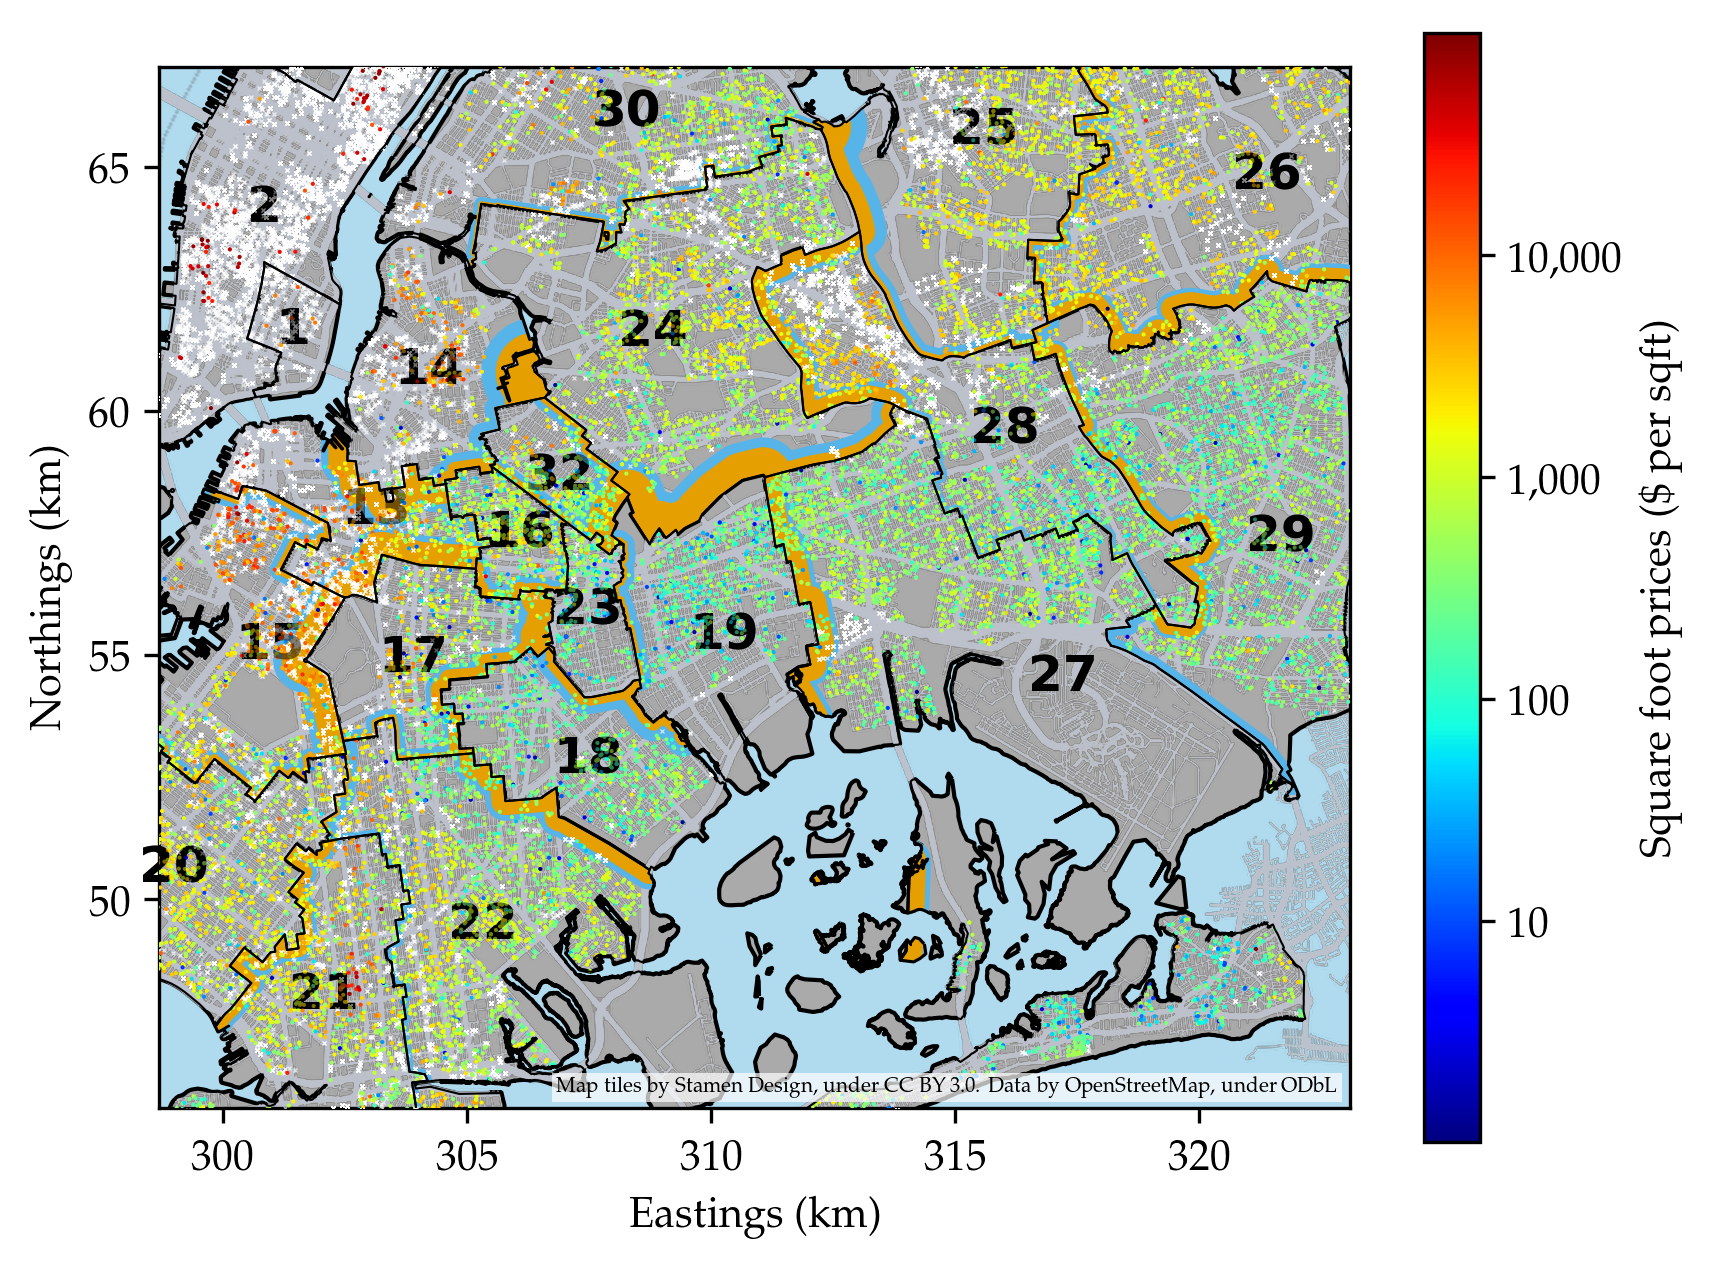
\includegraphics[width=0.97\textwidth,height=0.8\textheight,keepaspectratio]{figures/pairwise_mean_se.pdf}
    \caption[]{
		\label{fig:NYC_pairwise}
        \textbf{Pairwise estimates of the inverse variance LATE between adjacent districts.}
        The thickness of the orange buffer adjacent to borders is proportional to the posterior mean of the inverse variance LATE, and the blue buffer beyond it is proportional to the posterior standard deviation of the LATE.
    The buffers are drawn on the side of the border that is estimated to have higher house prices. 
        \\\hspace{\textwidth}
        \textbf{Background:} 
        Map of property sales in New York City. Each dot is a sale, and its color indicates the price per square foot. White crosses indicate sales of properties with missing square footage, which are therefore excluded from the analysis. School district boundaries are shown, and each district is labeled by its number.
    }
\end{figure}

	Some school districts are separated by parks (or other non-residential zones), for example districts 15 \& 17 or 19 \& 24, so that house sales do not extend all the way to the border on one or both sides.
A significant treatment effect between these pairs cannot be interpreted as the detection of a discontinuity in prices at the border, let alone any kind of causal interpretation, but rather it means that the difference in prices between the two sides of the park exceeds the typical spatial variation of house prices expected over the same distance.
This is not unsurprising, and one may speculate that physical barriers like parks, rivers, railways and major roads can separate neighborhoods with distinct character, demographics and thus house prices.
This in turn challenges the stationarity assumption of the spatial model \autorefexternal{eq:spec2gp}.
The higher distance between data and the border also stretches the spatial model's ability to extrapolate, which makes it more vulnerable to model misspecification.

	Other pairs of district, like 13 \& 14, 13 \& 17, and 25 \& 28 have clusters of missing data (condo sales with unknown square footage) near the border that cast doubt on the interpretation of the estimated effect.
Nonetheless, significant effects are also found between pairs of school districts without issues due to compound treatments, physical barriers, or missing data.
House prices increase going across the border from districts 16 to 13, 18 to 17, 24 to 30, 23 to 17, 25 to 26, 28 to 29, and 29 to 26.
Overall, it seems that school district borders in Brooklyn and Queens can correspond to measurable jumps in house prices per square foot.
The estimated size of this effect varies: zero or negligible in some cases, such as between districts 15, 20, 21, and 22; and quite pronounced in others, such as a 20\% price increase from 29 to 26, or 22\% from 18 to 17.

% \begin{landscape}
    % \begin{table}[p]
\begin{sidewaystable}
        \footnotesize
        \begin{tabular}{r|lllllll}
            \hline
\( \mathbf{13} \)& \( \mathbf{14:}~-0.29 \pm 0.09 \)& \( \mathbf{15:}~+0.03 \pm 0.07 \)& \( \mathbf{16:}~+0.13 \pm 0.07 \)& \( \mathbf{17:}~+0.26 \pm 0.08 \)\\ 
\( \mathbf{14} \)& \( \mathbf{13:}~-0.29 \pm 0.09 \)& \( \mathbf{16:}~+0.16 \pm 0.10 \)& \( \mathbf{24:}~+0.38 \pm 0.15 \)& \( \mathbf{32:}~+0.07 \pm 0.12 \)\\ 
\( \mathbf{15} \)& \( \mathbf{13:}~+0.03 \pm 0.07 \)& \( \mathbf{17:}~+0.18 \pm 0.10 \)& \( \mathbf{20:}~-0.05 \pm 0.06 \)& \( \mathbf{22:}~-0.28 \pm 0.11 \)\\ 
\( \mathbf{16} \)& \( \mathbf{13:}~+0.13 \pm 0.07 \)& \( \mathbf{14:}~+0.16 \pm 0.10 \)& \( \mathbf{17:}~-0.04 \pm 0.07 \)& \( \mathbf{23:}~-0.10 \pm 0.07 \)& \( \mathbf{32:}~-0.05 \pm 0.06 \)\\ 
\( \mathbf{17} \)& \( \mathbf{13:}~+0.26 \pm 0.08 \)& \( \mathbf{15:}~+0.18 \pm 0.10 \)& \( \mathbf{16:}~-0.04 \pm 0.07 \)& \( \mathbf{18:}~+0.20 \pm 0.07 \)& \( \mathbf{22:}~+0.06 \pm 0.07 \)& \( \mathbf{23:}~-0.29 \pm 0.10 \)\\ 
\( \mathbf{18} \)& \( \mathbf{17:}~+0.20 \pm 0.07 \)& \( \mathbf{19:}~-0.06 \pm 0.12 \)& \( \mathbf{22:}~+0.10 \pm 0.07 \)& \( \mathbf{23:}~-0.03 \pm 0.09 \)\\ 
\( \mathbf{19} \)& \( \mathbf{18:}~-0.06 \pm 0.12 \)& \( \mathbf{23:}~-0.00 \pm 0.08 \)& \( \mathbf{24:}~+0.39 \pm 0.11 \)& \( \mathbf{27:}~+0.19 \pm 0.06 \)& \( \mathbf{32:}~-0.27 \pm 0.12 \)\\ 
\( \mathbf{20} \)& \( \mathbf{15:}~-0.05 \pm 0.06 \)& \( \mathbf{21:}~-0.04 \pm 0.05 \)& \( \mathbf{22:}~+0.11 \pm 0.08 \)\\ 
\( \mathbf{21} \)& \( \mathbf{20:}~-0.04 \pm 0.05 \)& \( \mathbf{22:}~-0.04 \pm 0.05 \)\\ 
\( \mathbf{22} \)& \( \mathbf{15:}~-0.28 \pm 0.11 \)& \( \mathbf{17:}~+0.06 \pm 0.07 \)& \( \mathbf{18:}~+0.10 \pm 0.07 \)& \( \mathbf{20:}~+0.11 \pm 0.08 \)& \( \mathbf{21:}~-0.04 \pm 0.05 \)\\ 
\( \mathbf{23} \)& \( \mathbf{16:}~-0.10 \pm 0.07 \)& \( \mathbf{17:}~-0.29 \pm 0.10 \)& \( \mathbf{18:}~-0.03 \pm 0.09 \)& \( \mathbf{19:}~-0.00 \pm 0.08 \)& \( \mathbf{32:}~+0.04 \pm 0.08 \)\\ 
\( \mathbf{24} \)& \( \mathbf{14:}~+0.38 \pm 0.15 \)& \( \mathbf{19:}~+0.39 \pm 0.11 \)& \( \mathbf{25:}~-0.26 \pm 0.13 \)& \( \mathbf{27:}~-0.22 \pm 0.10 \)& \( \mathbf{28:}~+0.06 \pm 0.06 \)& \( \mathbf{30:}~-0.14 \pm 0.05 \)& \( \mathbf{32:}~-0.02 \pm 0.08 \)\\ 
\( \mathbf{25} \)& \( \mathbf{24:}~-0.26 \pm 0.13 \)& \( \mathbf{26:}~+0.08 \pm 0.04 \)& \( \mathbf{28:}~-0.15 \pm 0.08 \)& \( \mathbf{29:}~-0.06 \pm 0.10 \)& \( \mathbf{30:}~+0.28 \pm 0.15 \)\\ 
\( \mathbf{26} \)& \( \mathbf{25:}~+0.08 \pm 0.04 \)& \( \mathbf{29:}~-0.18 \pm 0.05 \)\\ 
\( \mathbf{27} \)& \( \mathbf{19:}~+0.19 \pm 0.06 \)& \( \mathbf{24:}~-0.22 \pm 0.10 \)& \( \mathbf{28:}~-0.04 \pm 0.04 \)& \( \mathbf{29:}~+0.01 \pm 0.08 \)\\ 
\( \mathbf{28} \)& \( \mathbf{24:}~+0.06 \pm 0.06 \)& \( \mathbf{25:}~-0.15 \pm 0.08 \)& \( \mathbf{27:}~-0.04 \pm 0.04 \)& \( \mathbf{29:}~-0.09 \pm 0.04 \)\\ 
\( \mathbf{29} \)& \( \mathbf{25:}~-0.06 \pm 0.10 \)& \( \mathbf{26:}~-0.18 \pm 0.05 \)& \( \mathbf{27:}~+0.01 \pm 0.08 \)& \( \mathbf{28:}~-0.09 \pm 0.04 \)\\ 
\( \mathbf{30} \)& \( \mathbf{24:}~-0.14 \pm 0.05 \)& \( \mathbf{25:}~+0.28 \pm 0.15 \)\\ 
\( \mathbf{32} \)& \( \mathbf{14:}~+0.07 \pm 0.12 \)& \( \mathbf{16:}~-0.05 \pm 0.06 \)& \( \mathbf{19:}~-0.27 \pm 0.12 \)& \( \mathbf{23:}~+0.04 \pm 0.08 \)& \( \mathbf{24:}~-0.02 \pm 0.08 \)\\ 
            \hline
        \end{tabular}
        \caption{
            \label{table:NYC_pairwise}
            \textbf{Estimated Treatment Effects Between Adjacent NYC School Districts.}
            Each row gives the posterior (mean \(\pm\) standard deviation) of the inverse-variance LATEs for one district (row header) compared to its neighbors.
            For example the first cell indicates an estimated average change in log house prices per square foot of -0.29 when crossing the border from district 13 to 14.
        }
\end{sidewaystable}
    % \end{table}
% \end{landscape}


% \bibliographystyle{chicago}
% \bibliography{GeoRDD}

\end{document}
